%&pdflatex
\documentclass[final,leqno]{siamltex}
%\documentclass[10pt,onecolumn]{article}
\usepackage[top=2cm,bottom=3cm,left=3.5cm,right=3.5cm]{geometry}
\usepackage[utf8]{inputenc}
\usepackage{amsmath,amssymb,amsfonts,mathrsfs}
\let\proof\relax 
\let\endproof\relax
\usepackage{amsthm}
\usepackage{amssymb}
\usepackage{amscd}
\usepackage{listings}
\usepackage{array}
\usepackage{mathtools}
\usepackage{dsfont}
\usepackage{graphicx}
\usepackage{pdfpages}
\usepackage[textsize=footnotesize,color=green]{todonotes}
\usepackage{algorithm, algorithmic}
\usepackage{array}
\usepackage{bm}
\usepackage{tikz}
\usepackage{subfigure}
\usepackage[normalem]{ulem}

\newcommand{\bs}[1]{\boldsymbol{#1}}

\newcommand{\equaldef}{\stackrel{\mathrm{def}}{=}}

\newcommand{\tablab}[1]{\label{tab:#1}}
\newcommand{\tabref}[1]{Table~\ref{tab:#1}}

\newcommand{\theolab}[1]{\label{theo:#1}}
\newcommand{\theoref}[1]{\ref{theo:#1}}
\newcommand{\eqnlab}[1]{\label{eq:#1}}
\newcommand{\eqnref}[1]{\eqref{eq:#1}}
\newcommand{\seclab}[1]{\label{sec:#1}}
\newcommand{\secref}[1]{\ref{sec:#1}}
\newcommand{\lemlab}[1]{\label{lem:#1}}
\newcommand{\lemref}[1]{\ref{lem:#1}}

\newcommand{\mb}[1]{\mathbf{#1}}
\newcommand{\mbb}[1]{\mathbb{#1}}
\newcommand{\mc}[1]{\mathcal{#1}}
\newcommand{\nor}[1]{\left\| #1 \right\|}
\newcommand{\snor}[1]{\left| #1 \right|}
\newcommand{\LRp}[1]{\left( #1 \right)}
\newcommand{\LRs}[1]{\left[ #1 \right]}
\newcommand{\LRa}[1]{\left\langle #1 \right\rangle}
\newcommand{\LRc}[1]{\left\{ #1 \right\}}
\newcommand{\LRb}[1]{\left| #1 \right|}

\newcommand{\tanbui}[2]{\textcolor{blue}{\sout{#1}} \textcolor{red}{#2}}
\newcommand{\Grad} {\ensuremath{\nabla}}
\newcommand{\Div} {\ensuremath{\nabla\cdot}}
\newcommand{\Nel} {\ensuremath{{N^\text{el}}}}
\newcommand{\jump}[1] {\ensuremath{\LRs{\!\left[#1\right]\!}}}
\newcommand{\uh}{\widehat{u}}
\newcommand{\fnh}{\widehat{f}_n}
\renewcommand{\L}{L^2\LRp{\Omega}}
\newcommand{\pO}{\partial\Omega}
\newcommand{\Gh}{\Gamma_h}
\newcommand{\Gm}{\Gamma_{-}}
\newcommand{\Gp}{\Gamma_{+}}
\newcommand{\Go}{\Gamma_0}
\newcommand{\Oh}{\Omega_h}

\newcommand{\eval}[2][\right]{\relax
  \ifx#1\right\relax \left.\fi#2#1\rvert}

\def\etal{{\it et al.~}}

\newcommand{\vect}[1]{\ensuremath\boldsymbol{#1}}
\newcommand{\tensor}[1]{\underline{\vect{#1}}}
\newcommand{\del}{\Delta}
\let\grad\relax
\newcommand{\grad}{\nabla}
\newcommand{\curl}{\grad \times}
\renewcommand{\div}{\grad \cdot}
\newcommand{\ip}[1]{\left\langle #1 \right\rangle}
\newcommand{\eip}[1]{a\left( #1 \right)}
\newcommand{\pd}[2]{\frac{\partial#1}{\partial#2}}
\newcommand{\pdd}[2]{\frac{\partial^2#1}{\partial#2^2}}

\newcommand{\circone}{\ding{192}}
\newcommand{\circtwo}{\ding{193}}
\newcommand{\circthree}{\ding{194}}
\newcommand{\circfour}{\ding{195}}
\newcommand{\circfive}{\ding{196}}

\def\arr#1#2#3#4{\left[
\begin{array}{cc}
#1 & #2\\
#3 & #4\\
\end{array}
\right]}
\def\vecttwo#1#2{\left[
\begin{array}{c}
#1\\
#2\\
\end{array}
\right]}
\def\vectthree#1#2#3{\left[
\begin{array}{c}
#1\\
#2\\
#3\\
\end{array}
\right]}
\def\vectfour#1#2#3#4{\left[
\begin{array}{c}
#1\\
#2\\
#3\\
#4\\
\end{array}
\right]}

%\newtheorem{proposition}{Proposition}
%\newtheorem{corollary}{Corollary}
%\newtheorem{theorem}{Theorem}
%\newtheorem{lemma}{Lemma}

\newcommand{\G} {\Gamma}
\newcommand{\Gin} {\Gamma_{in}}
\newcommand{\Gout} {\Gamma_{out}}

\newtheorem{remark}{Remark}

\title{Notes on $C_0$ DPG methods}
\author{Jesse Chan, John A. Evans}
\date{}
\begin{document}

\maketitle

\section{Uzawa vs matrix-free methods}
We have a saddle point problem 
\[
\arr{R_V}{B}{B^T}{0}\vecttwo{e}{u} = \vecttwo{f}{0}
\]
Assumptions: 
\begin{itemize}
\item We want to avoid solving the saddle point problem (indefinite, large)
\item We cannot form the Schur complement 
\[
S = B^T R_V^{-1} B
\]
as it's completely dense due to the globally coupled nature of $R_V^{-1}$.
\end{itemize}
The two methods left are matrix-free methods for solving $Su = f$ and inexact Uzawa algorithms for the saddle point problem.  Each method relies heavily on the assumption that $R_V$ is easily invertible (the coercive and positive-definite nature of the operator should lend itself well to fast CG and multigrid-based solvers).  

The inexact Uzawa method is for the DPG saddle point problem
\begin{align*}
e_{i+1} &= e_i + \tilde{R_V}^{-1}\LRp{f - R_V e_i + B u_i}\\
u_{i+1} &= u_i + \tilde{S}^{-1}\LRp{B^T e}
\end{align*}
where $\tilde{S}^{-1}$ and $\tilde{R_V}^{-1}$ are meant to approximate the inverses of $R_V$ and $S$.  We assume for now that $\tilde{R_V}^{-1}$ is computable exactly, which gives us
\begin{align*}
e_{i+1} &= R_V^{-1}(f - Bu_i)\\
u_{i+1} &= u_i + \tilde{S}^{-1}\LRp{B^T e_i}.
\end{align*}
It can be shown that for the Uzawa iteration error $E_i = u-u_i$,
\[
E_{i+1} = \LRp{I-\tilde{S}^{-1}B^TR_V^{-1}B}E_i.
\]
If $\tilde{S}^{-1}$ is computed exactly as $S^{-1}$, the Uzawa method essentially reduces down to a matrix-free method, where the difficulty of the method becomes in preconditioning ${S}$ effectively.  The benefit of the Uzawa algorithm compared to matrix-free methods is the relaxation of the preconditioning required on $\tilde{S}$, in return for more iterations of the Uzawa algorithm loop.  


%\begin{figure}
%\centering
%\subfigure[No preconditioning]{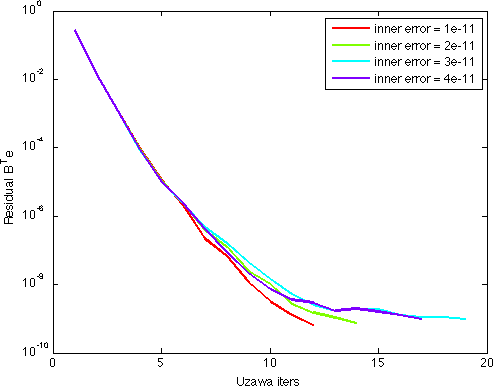
\includegraphics[width = .475\textwidth]{figs/uzawaInnerTol.png}}
%\subfigure[Diagonal preconditioning]{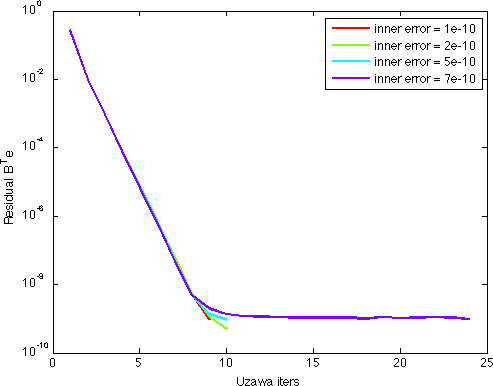
\includegraphics[width = .475\textwidth]{figs/uzawaDiagonalPreconditioning.png}}
%\end{figure}
%For an example of this, consider an Uzawa algorithm where $\tilde{S}$ is inverted by using non-preconditioned CG, with an error tolerance of $.1$ and a maximum of 25 iterations --- i.e. a very poor approximation of $S^{-1}$.  The exact solve for $R_V^{-1}$ is perturbed by random errors of order $10^-{11}$ to $4 \times 10^{-11}$.  Uzawa converges despite the poor choice of $\tilde{S}^{-1}$, but becomes very sensitive to inner iteration error, and stagnates at around $5\times 10^{-11}$.  By solving $S^{-1}$ more effectively (requiring a better preconditioner), we can afford a small error in our inner iteration.  Diagonal preconditioning for $S$, for example, converges to a solution for larger perturbations of $O(10^{-10}$ before stagnating at $7 \times 10^{-10}$.  
%
%Since the inner iteration will likely need to be solved inexactly as well, we'll likely need a better preconditioner for $S$, but i have no idea how you would precondition a completely dense matrix...

\end{document}
